\begin{frame}
    \frametitle{Mining and Consensus}
    \begin{block}{Definition}
        Mining \alert{secures} the bitcoin system and enables the emergence of network-wide \alert{consensus} without a \alert{central authority}. The reward of newly mined coins and transaction fees is an \alert{incentive scheme} that aligns the actions of miners with the \alert{security of the network}, while simultaneously implementing the \alert{monetary supply}.
    \end{block}
    \begin{figure}[htbp]
        \subfigure{
        \begin{minipage}[b]{0.45\textwidth}
            \centering
            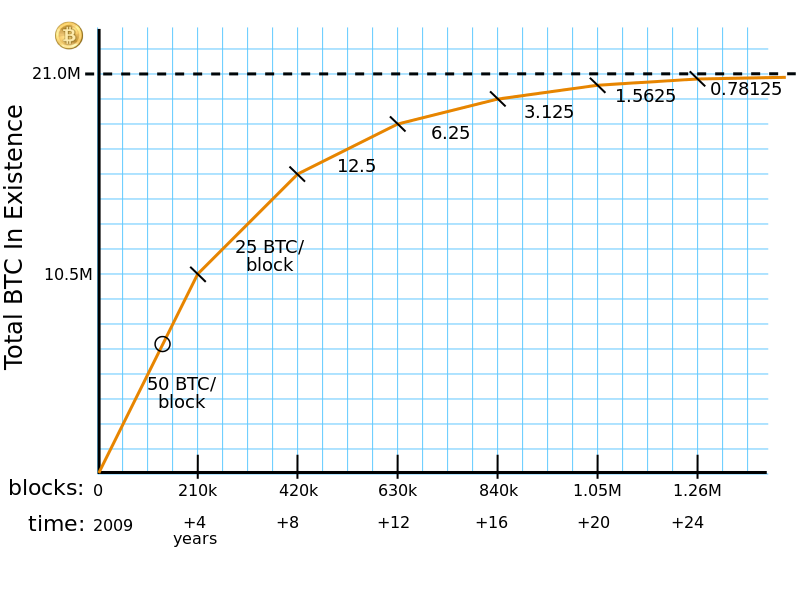
\includegraphics[scale=0.2]{mining-reward.png}
        \end{minipage}
    }
        \subfigure{
        \begin{minipage}[b]{0.45\textwidth}
            \centering
            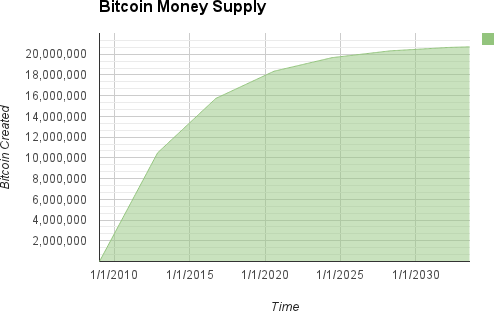
\includegraphics[scale=0.6]{mbc2_1001.png}
        \end{minipage}
    }
    \end{figure}
\end{frame}

\begin{frame}
    \frametitle{Decentralize Consensus}
    When there is no central authority, how can everyone in the network realize consensus?
    \begin{itemize}
        \item \textbf{tradition consensus algorithm}
            \begin{itemize}
                \item Paxos, Raft, \ldots
                \item Failure model: Not Byzantine(Node may fail, But not malicious)
                \item Leader election.
                \item Focusing on log(database), more universe
            \end{itemize}
        \item \textbf{blockchain consensus algorithm}
            \begin{itemize}
                \item PoW, PoS(Proof of Stake), \ldots
                \item Failure model: Byzantine(Node may be malicious)
                \item No election.
                \item Focusing on transaction.
            \end{itemize}
    \end{itemize}
    Anyway, all the consensus algorithm comply with the \alert{majority rule}.
\end{frame}

\begin{frame}
    \frametitle{Byzantine Generals' Problem}
    Story background:
    \begin{itemize}
        \item Generals of army surround enemy city
        \item Actions in union required to win
        \item Some generals may be traitors
        \item Messengers are reliable
    \end{itemize}
    \begin{center}
        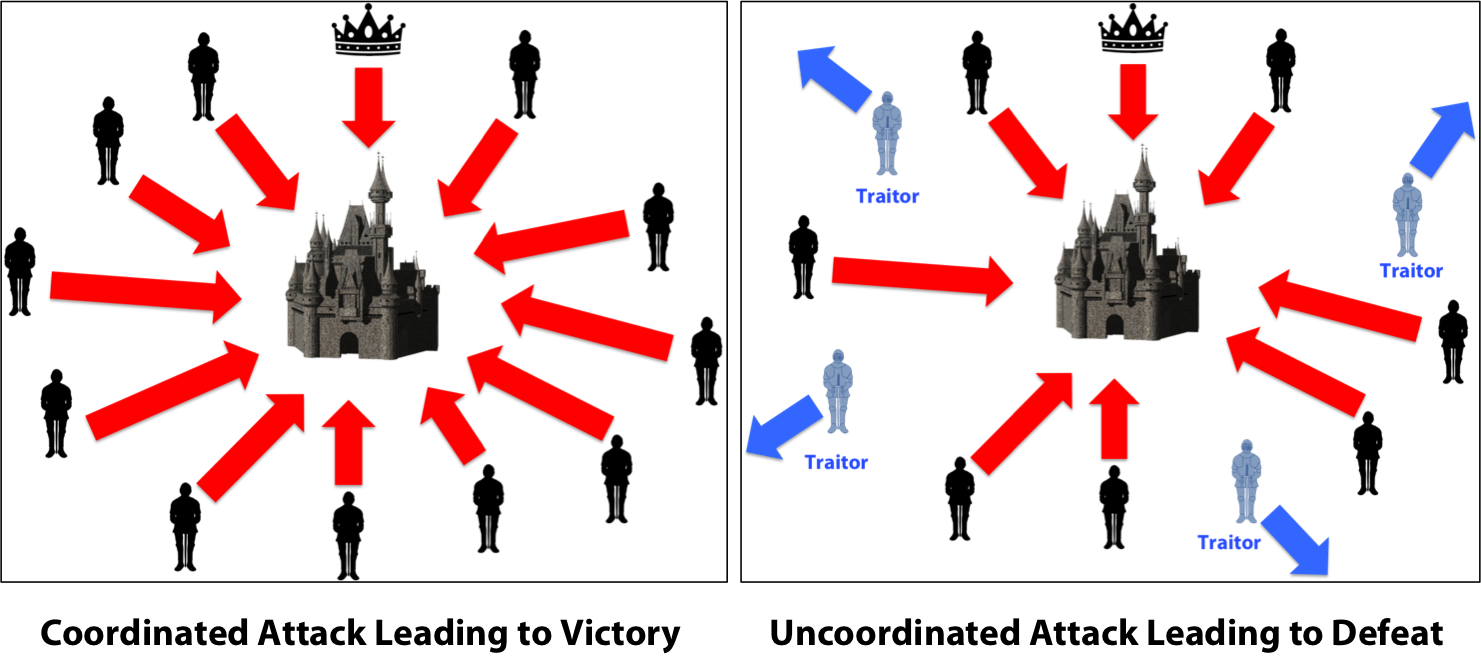
\includegraphics[scale=0.15]{byzantine-generals-problem.png}
    \end{center}
%    Results:
%    \begin{itemize}
%        \item No solution exists if less than or equal to 2/3 generals are loyal.
%    \end{itemize}
\end{frame}

\begin{frame}
    \frametitle{Proof of Work}
    \begin{itemize}
        \item \textbf{Fork}
            \begin{itemize}
                \item when 2 miners mine a block at the same time.
            \end{itemize}
        \item \textbf{Orphan}
            \begin{itemize}
                \item Only one can be in the chain, the other is called \alert{Orphan}
            \end{itemize}
        \item \textbf{Fork/Dispute Resolution}
            \begin{itemize}
                \item The longest block chain is valid.
            \end{itemize}
    \end{itemize}
    \begin{center}
        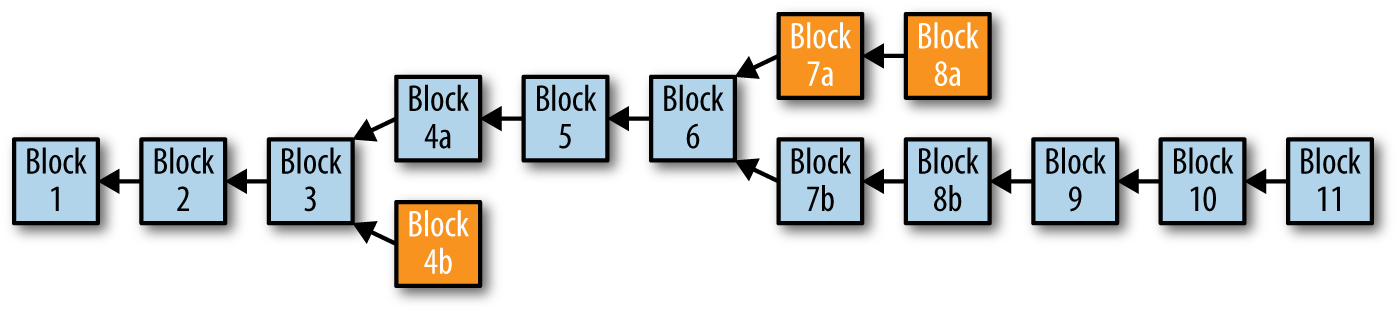
\includegraphics[scale=0.5]{mbc2_1009.png}
    \end{center}
\end{frame}

\begin{frame}
    \frametitle{Block Chain Fork}
    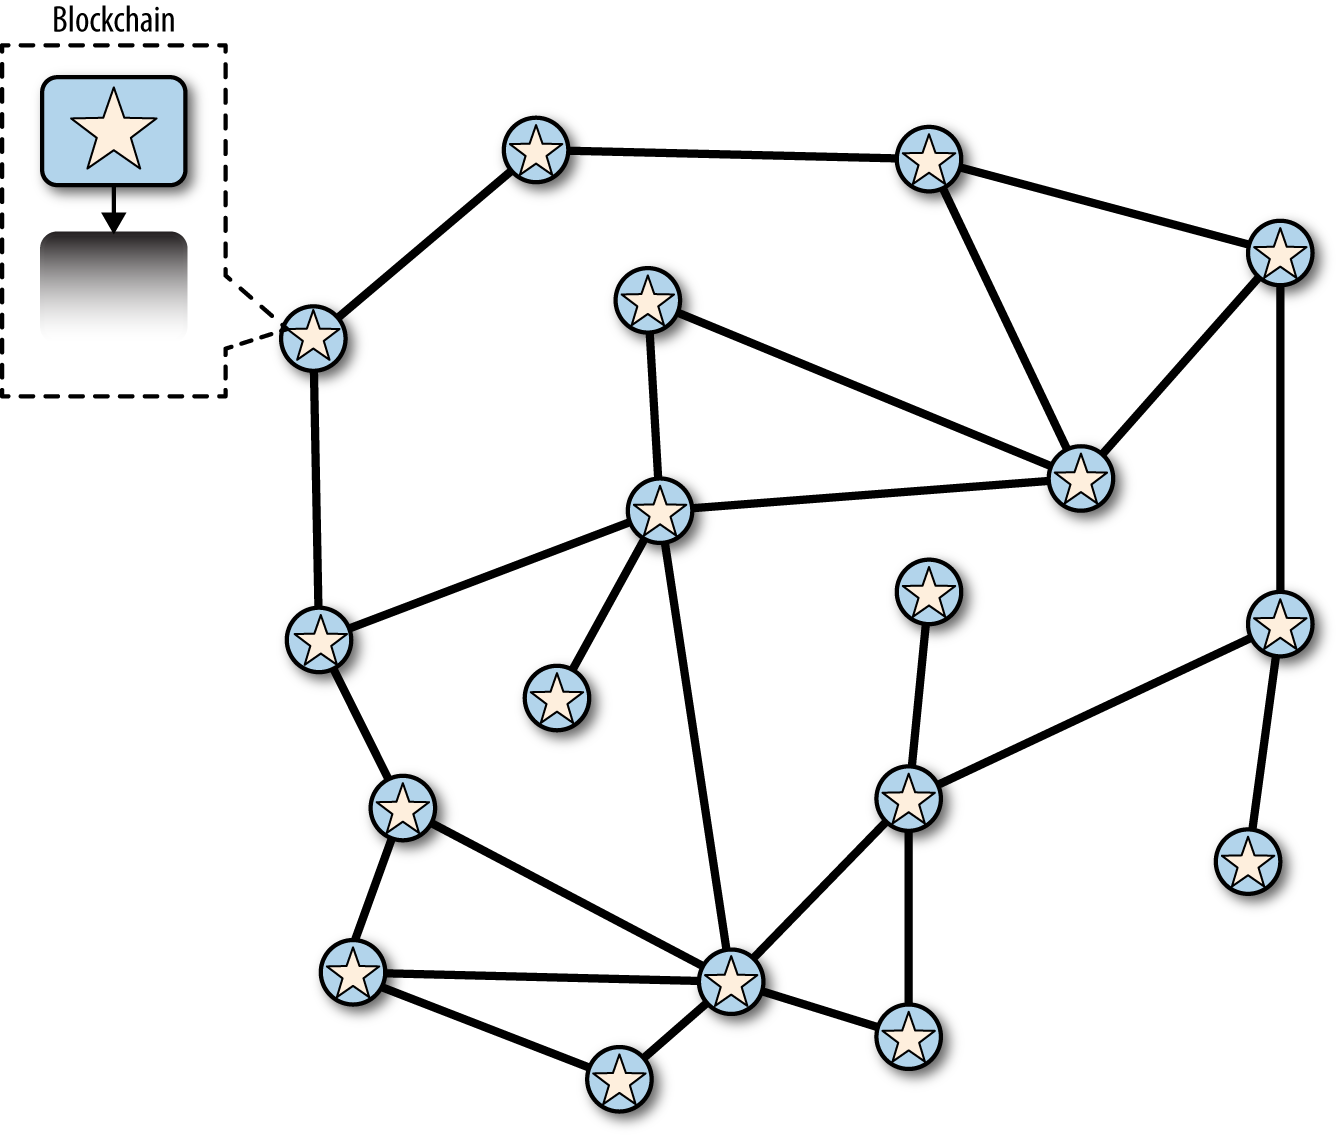
\includegraphics[scale=0.7]{mbc2_1002.png}
\end{frame}

\begin{frame}
    \frametitle{Block Chain Fork}
    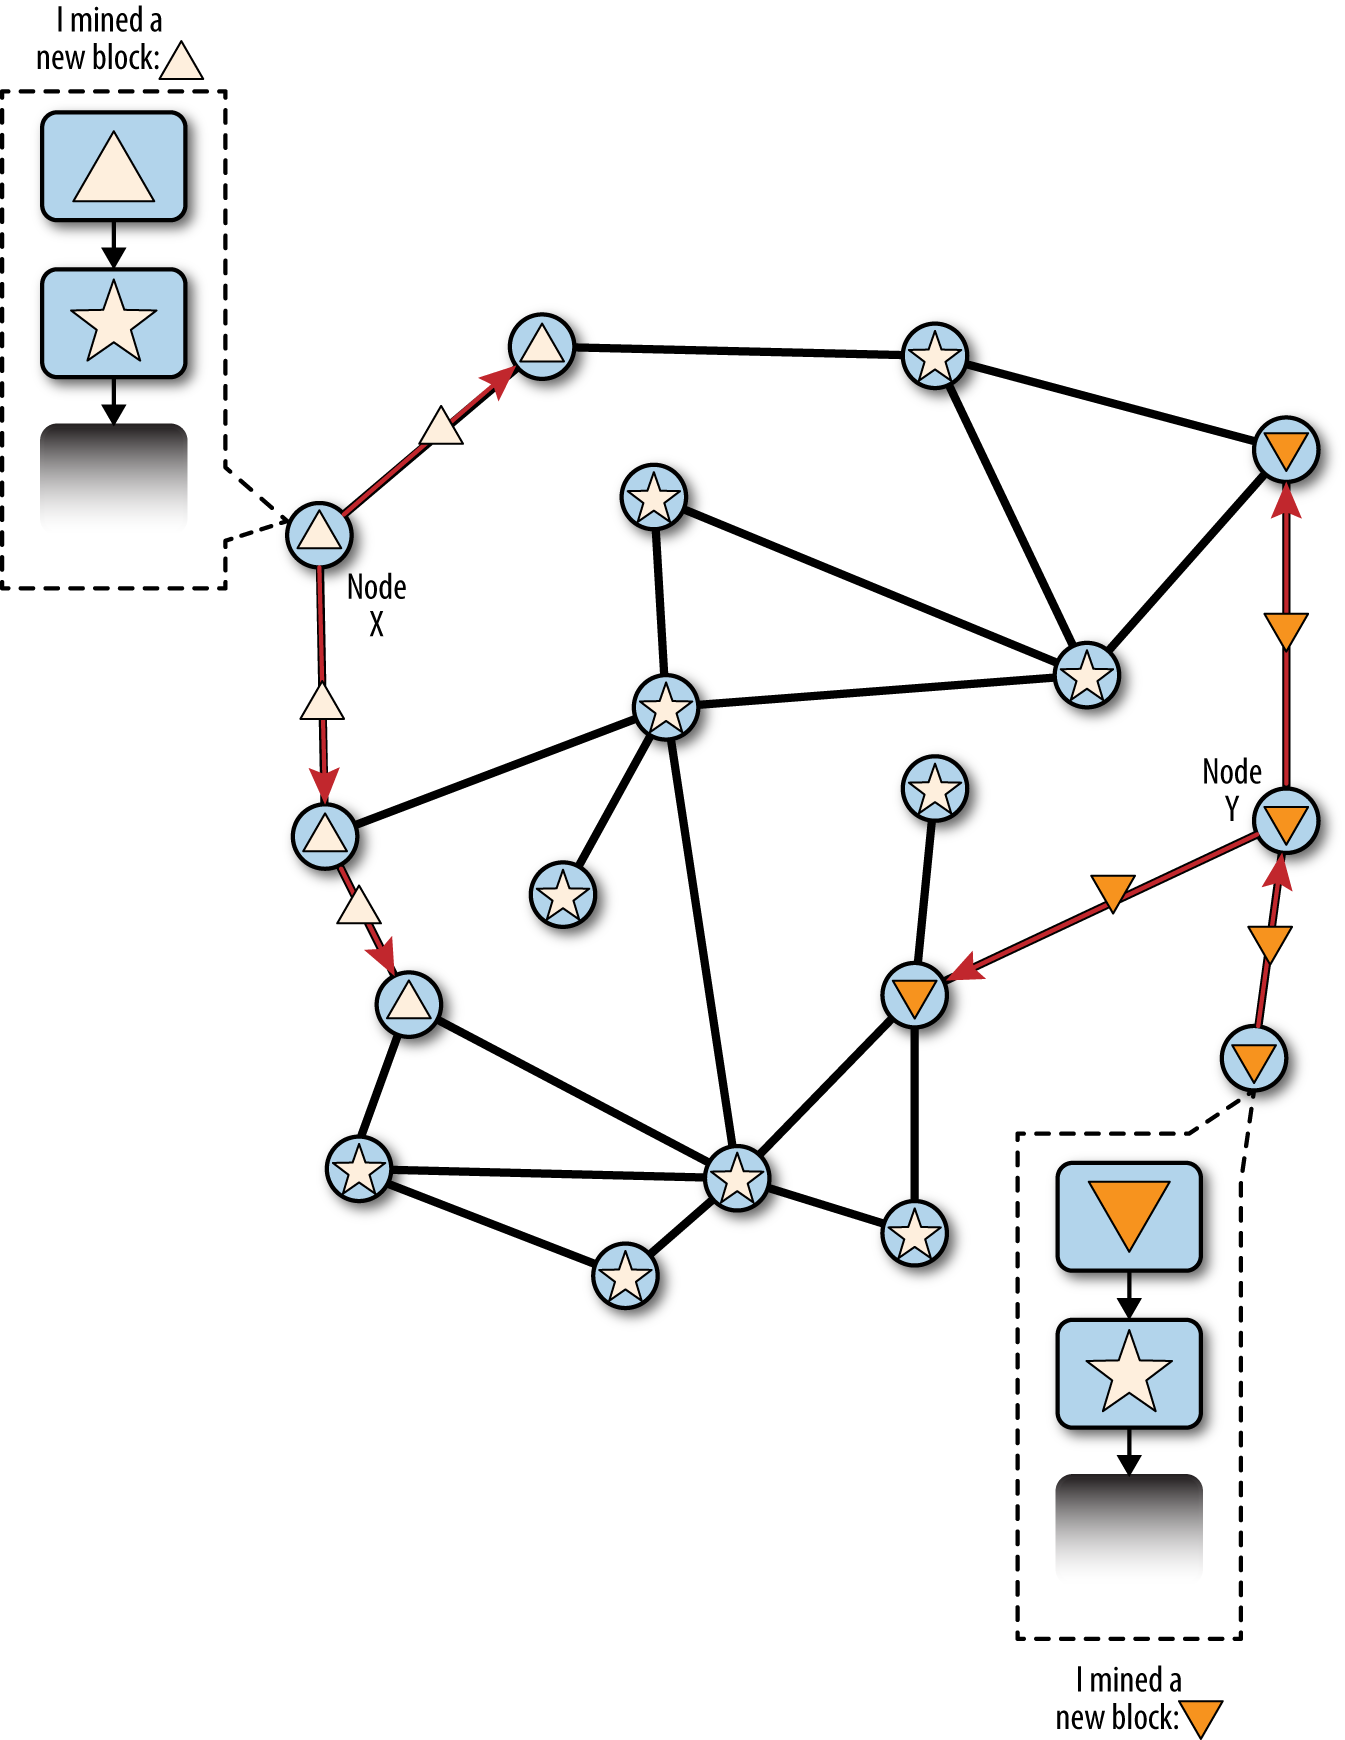
\includegraphics[scale=0.5]{mbc2_1003.png}
\end{frame}

\begin{frame}
    \frametitle{Block Chain Fork}
    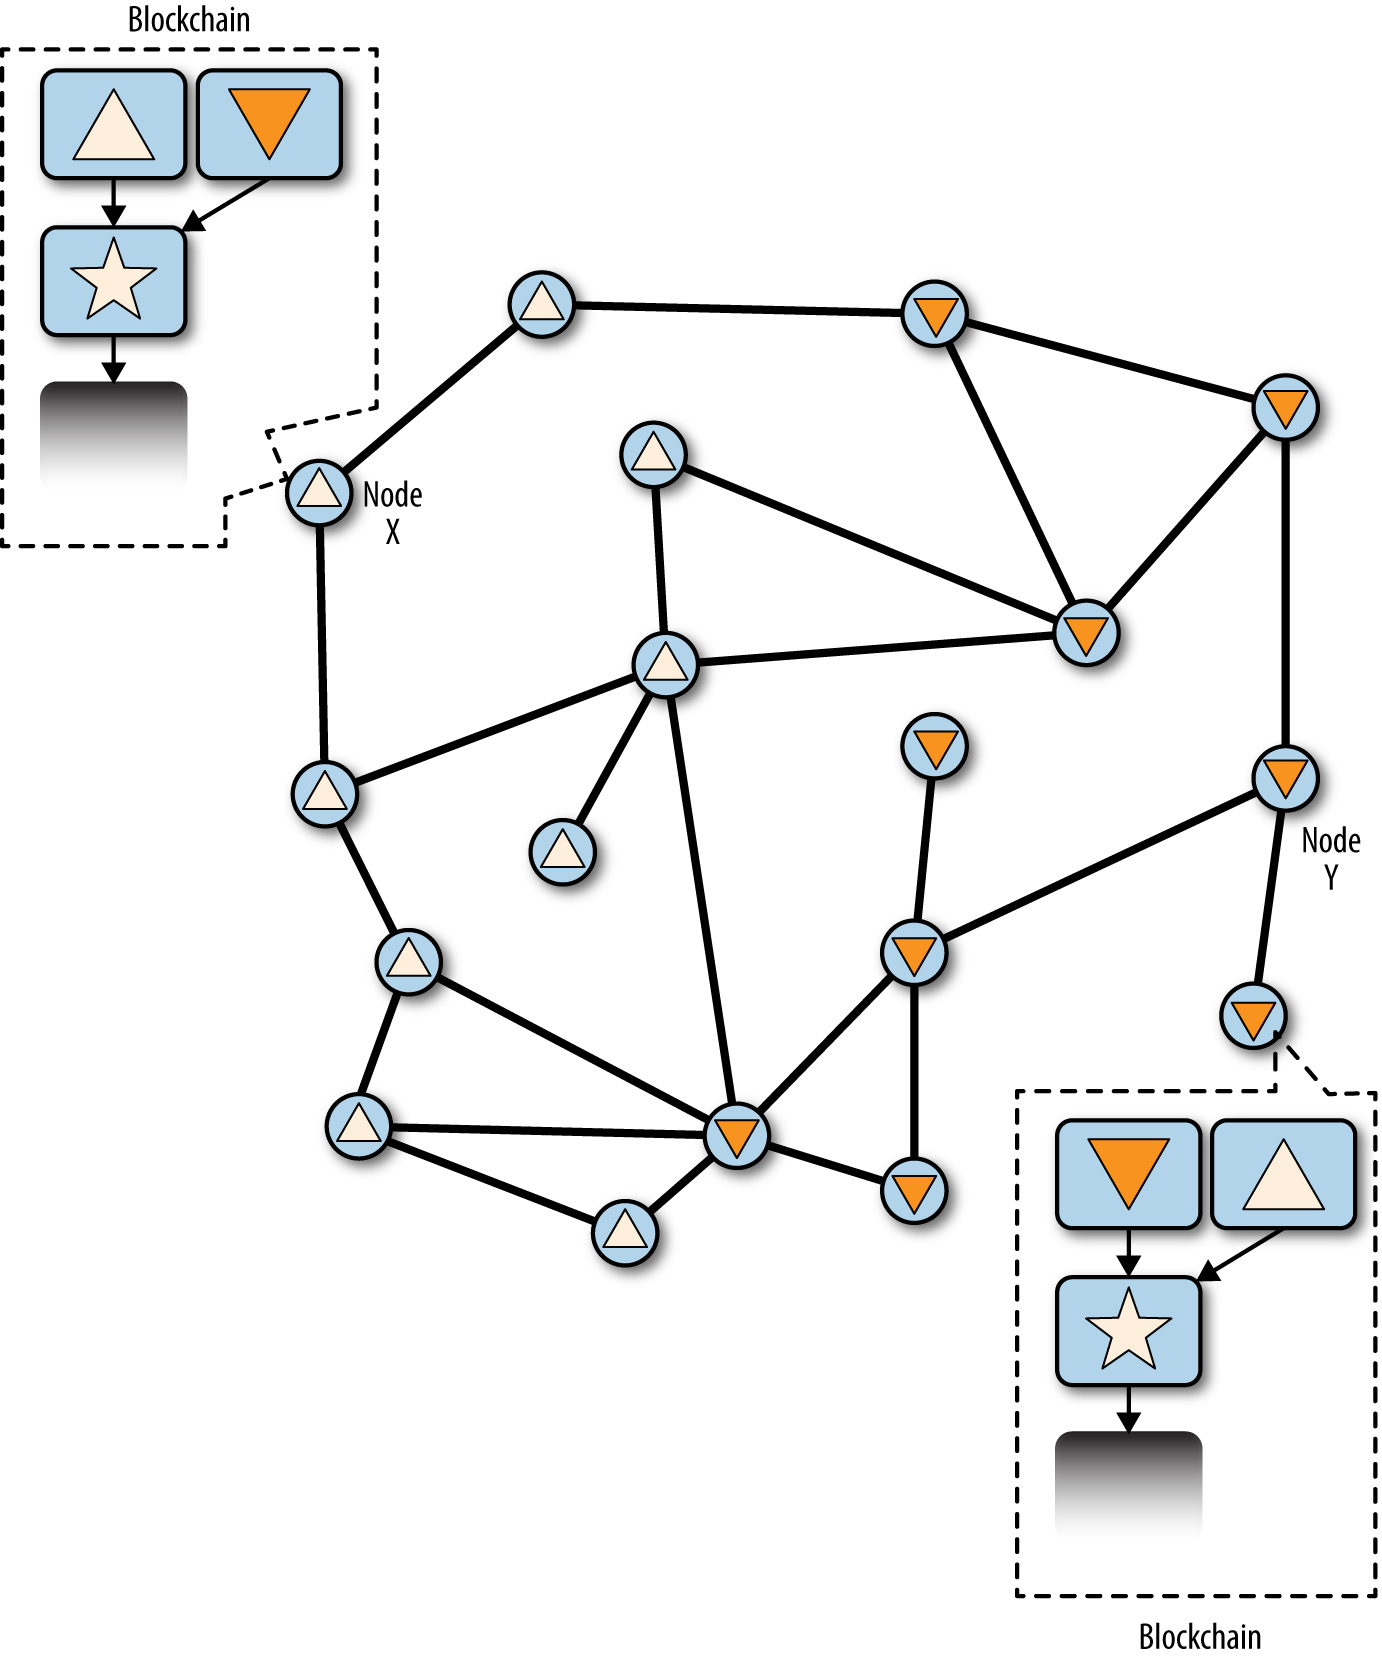
\includegraphics[scale=0.5]{mbc2_1004.png}
\end{frame}

\begin{frame}
    \frametitle{Block Chain Fork}
    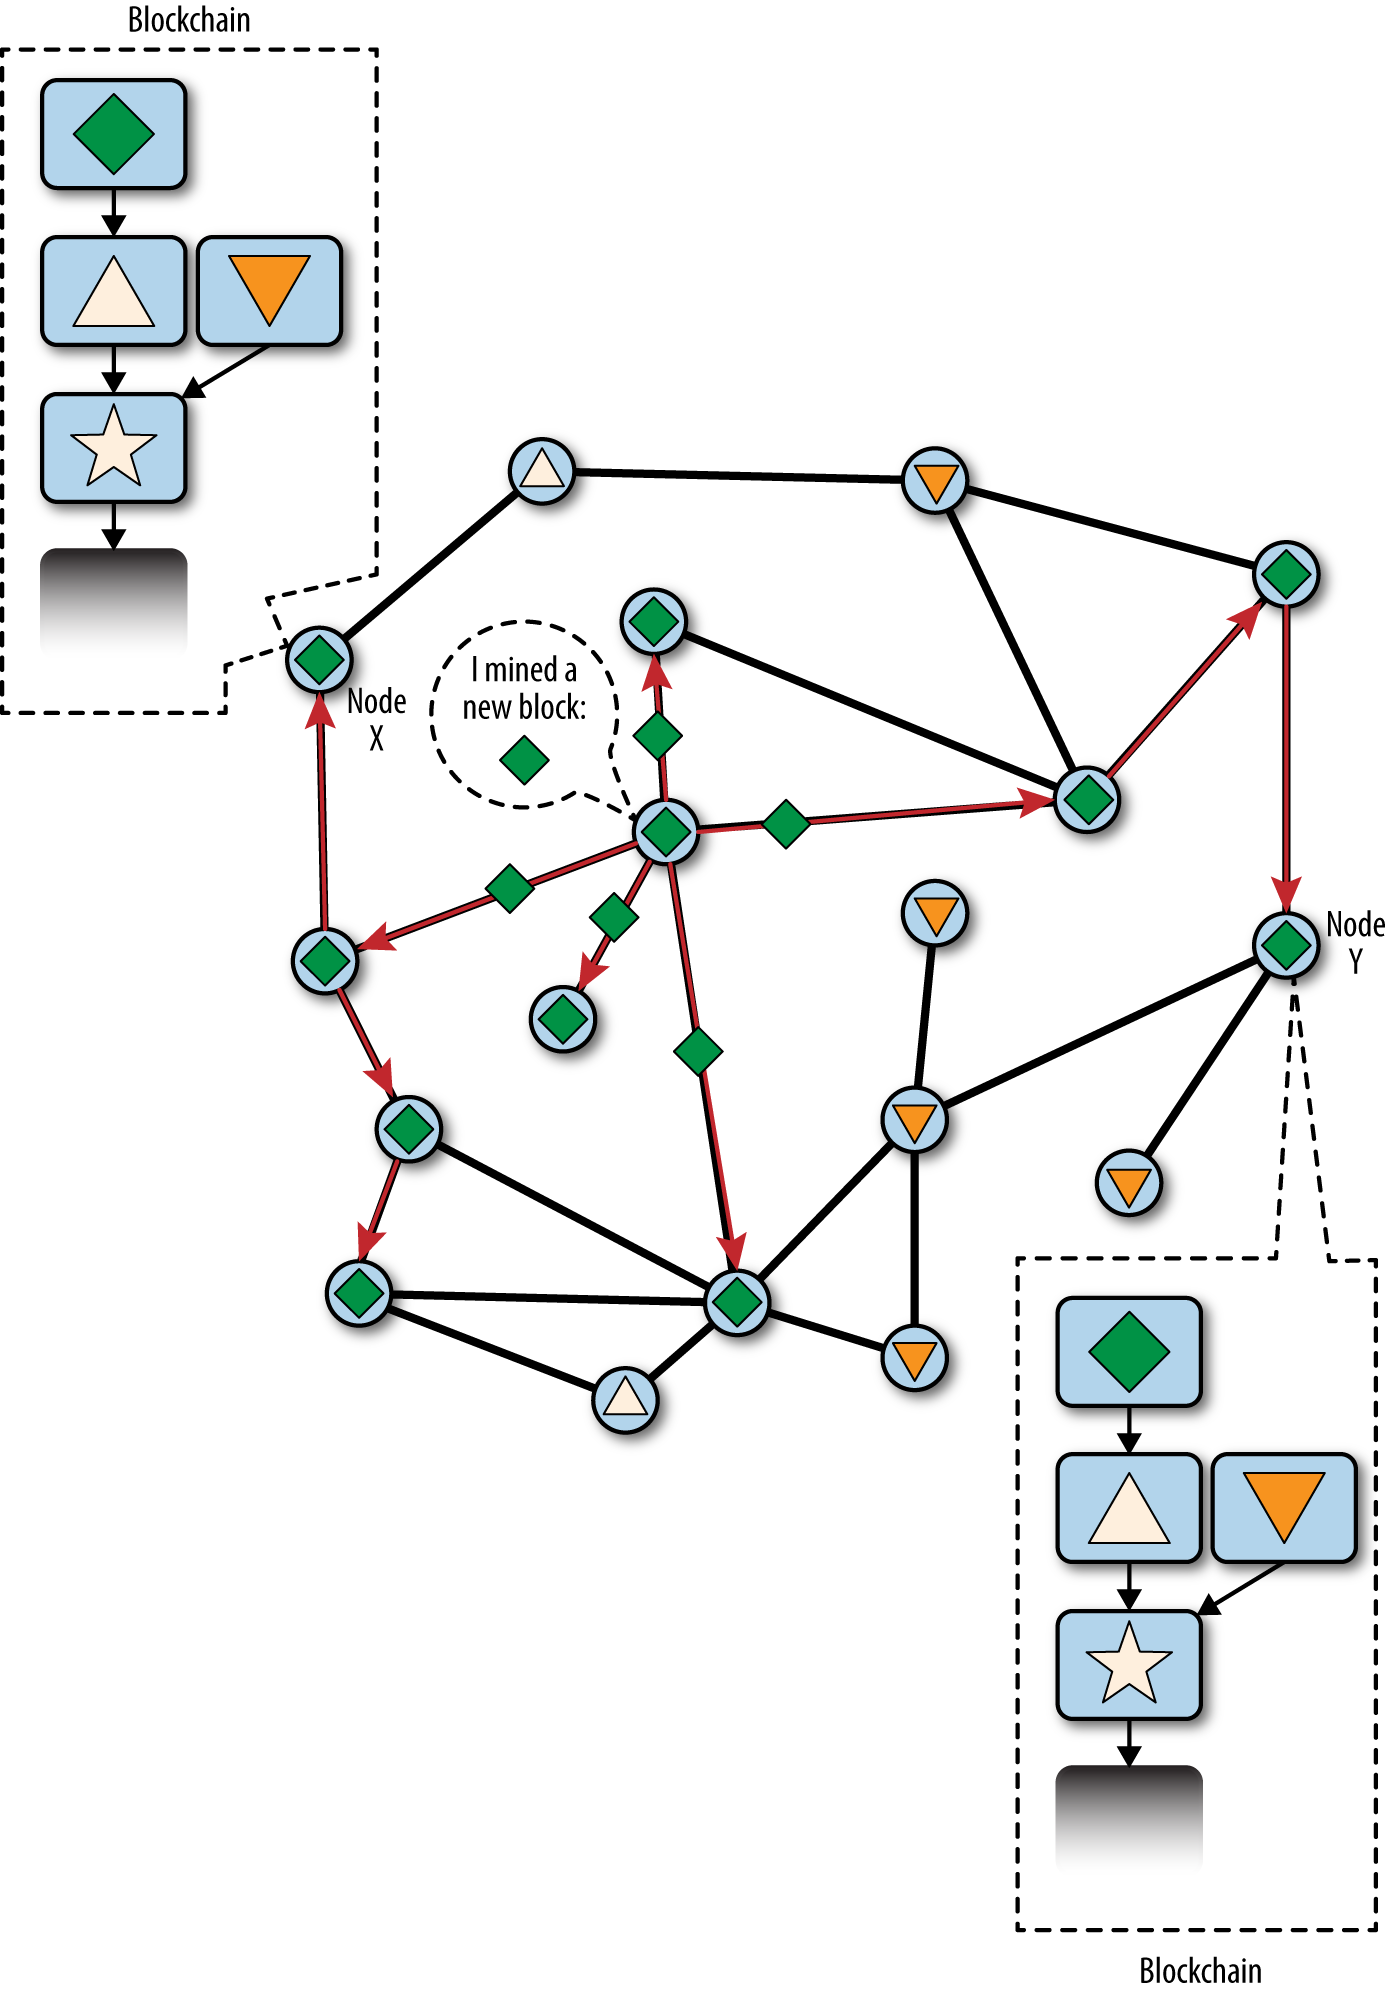
\includegraphics[scale=0.5]{mbc2_1005.png}
\end{frame}

\begin{frame}
    \frametitle{Block Chain Fork}
    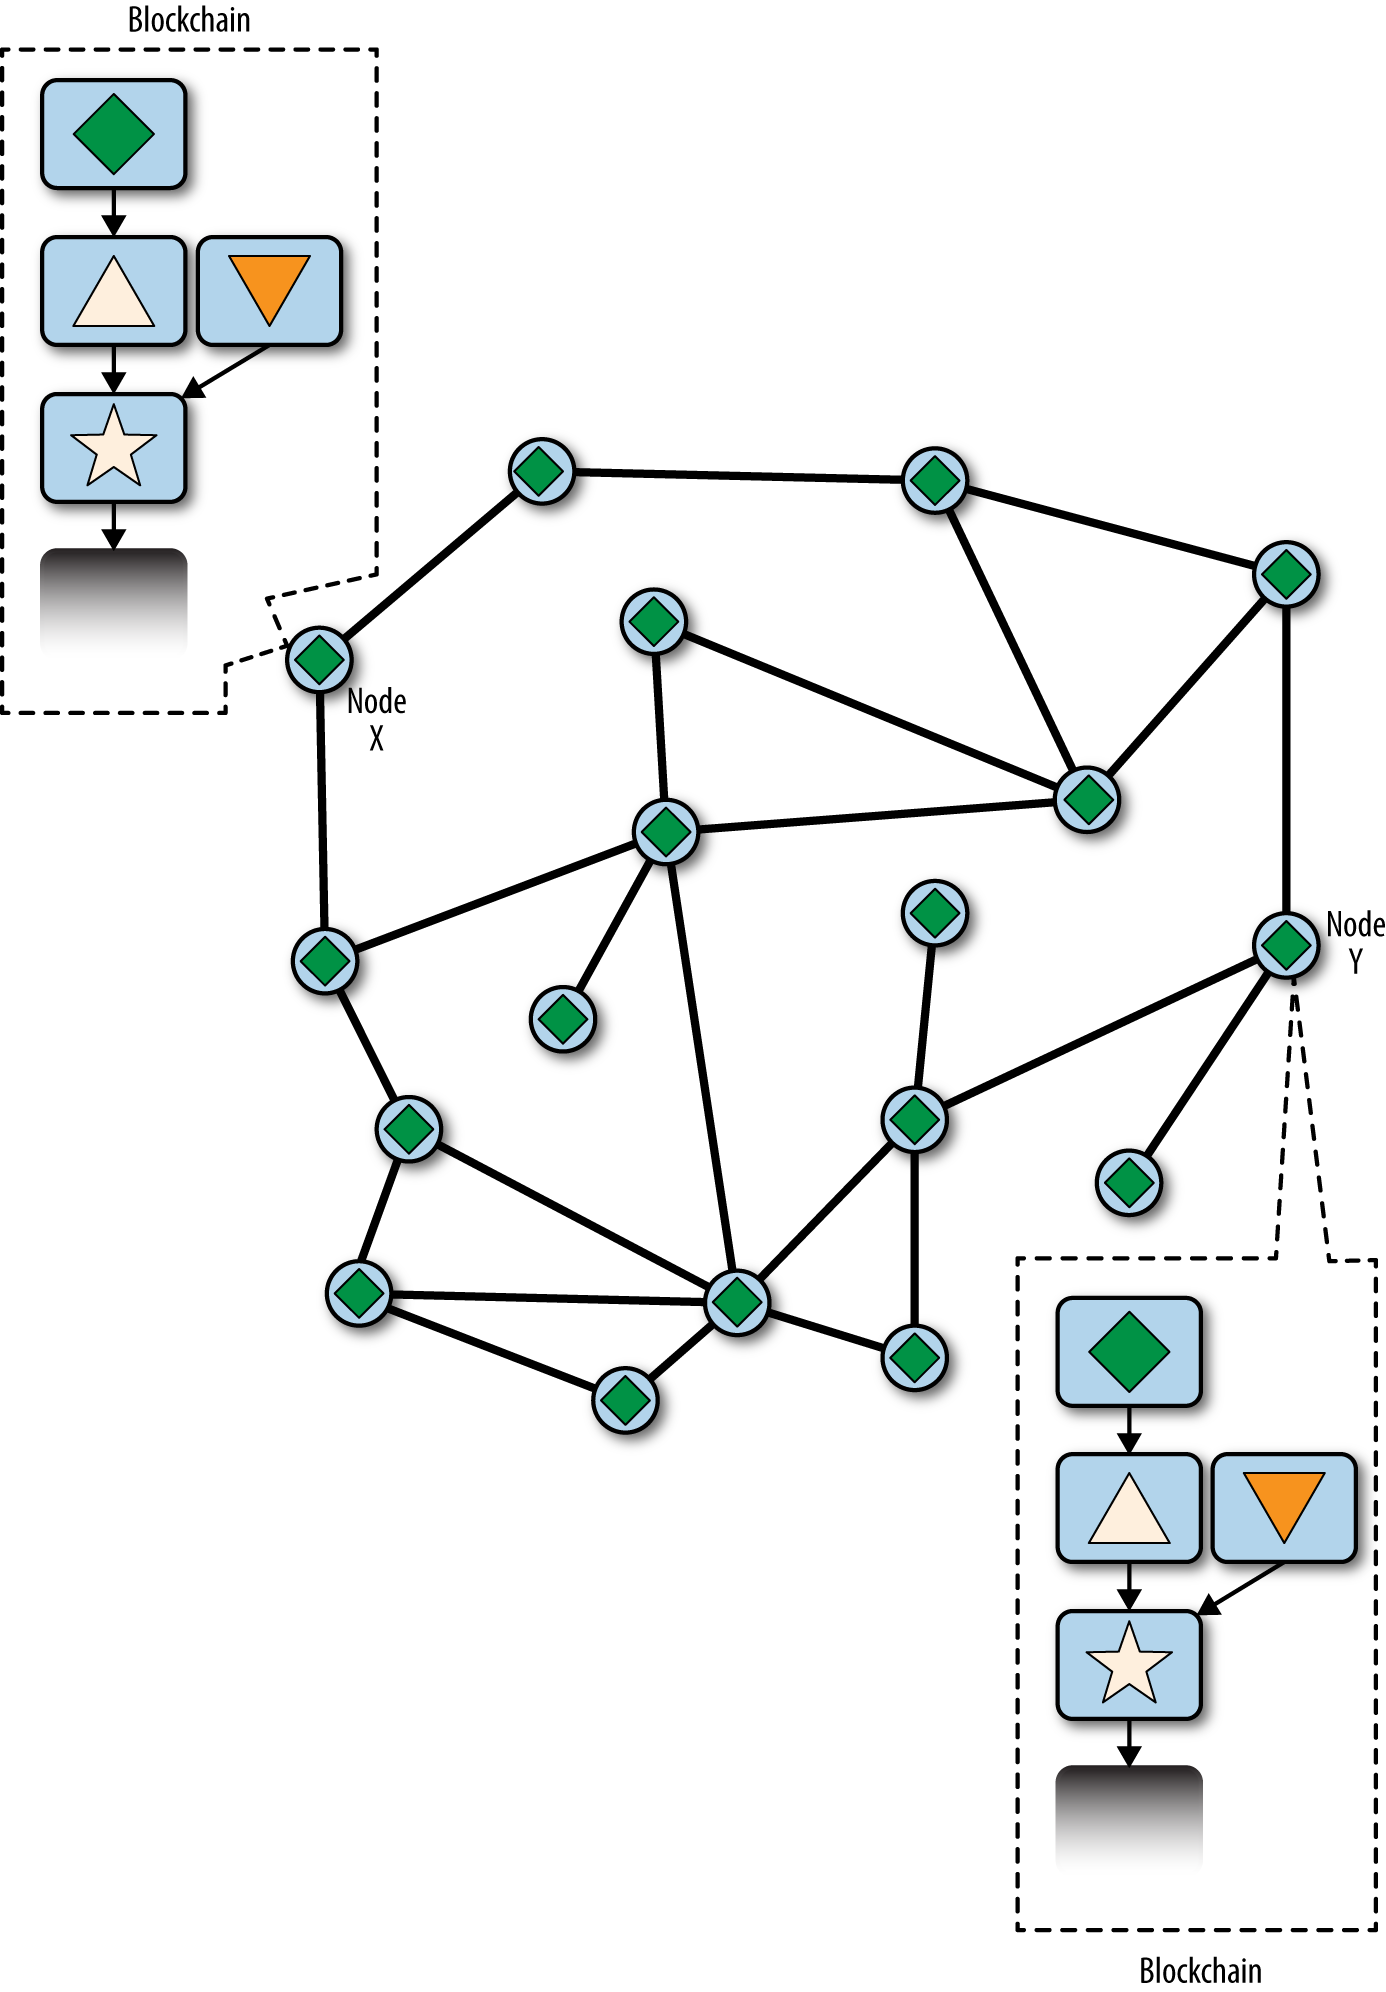
\includegraphics[scale=0.5]{mbc2_1006.png}
\end{frame}

\begin{frame}
    \frametitle{Double Spending Attack}
    Any attacker is competing against the whole network.
    \begin{center}
        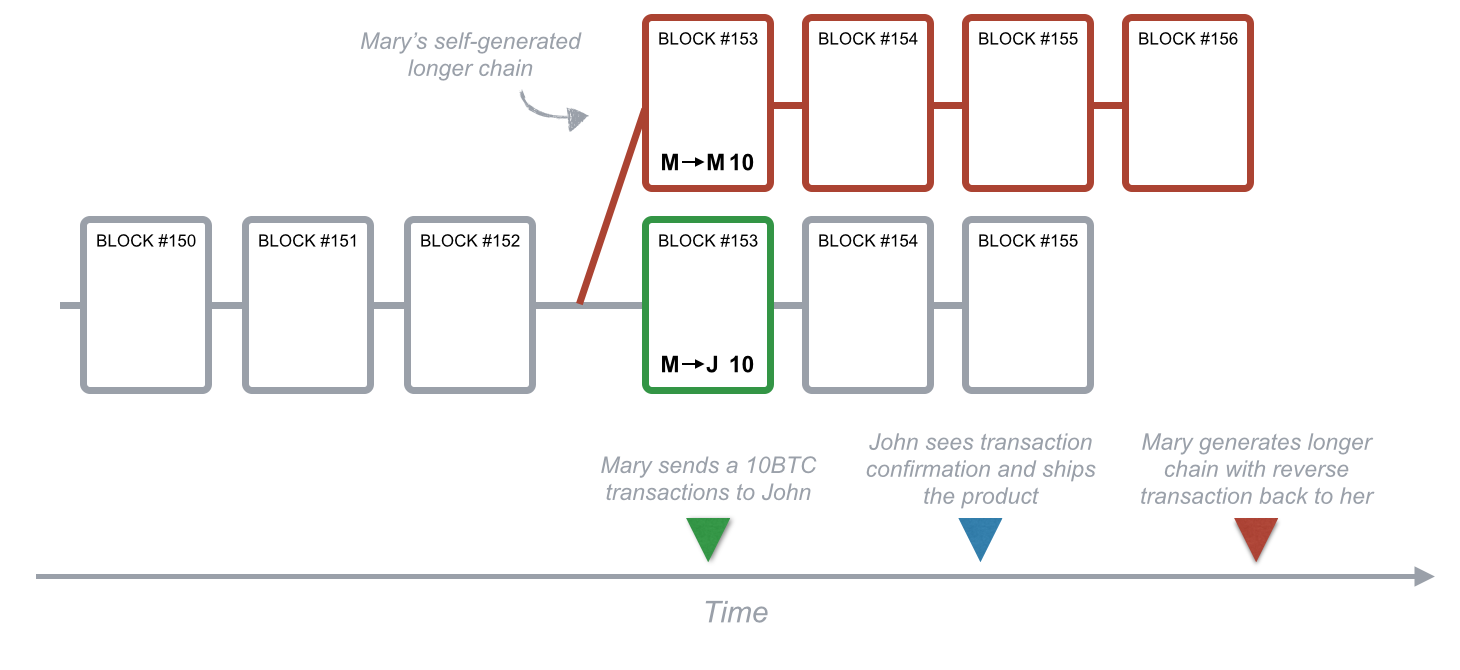
\includegraphics[scale=0.16]{double-spending.png}
    \end{center}
    \begin{itemize}
        \item Each block contains a reference to the previous block.
        \item 51\% computing power of the whole network have a 50\% chance to solve a block before some other node does.
        \item Create 2, 3 or more blocks in a row is even harder.
    \end{itemize}
\end{frame}

\begin{frame}
    \frametitle{Blockchain Transactions Security}
    Transactions get more and more secure with time.
    \begin{itemize}
        \item A block is add to the chain every 10 minutes on average.
        \item Waiting for 6 block(1 hour) gives a quite high probability that the transaction has been processed and is \alert{non reversible}.
    \end{itemize}
    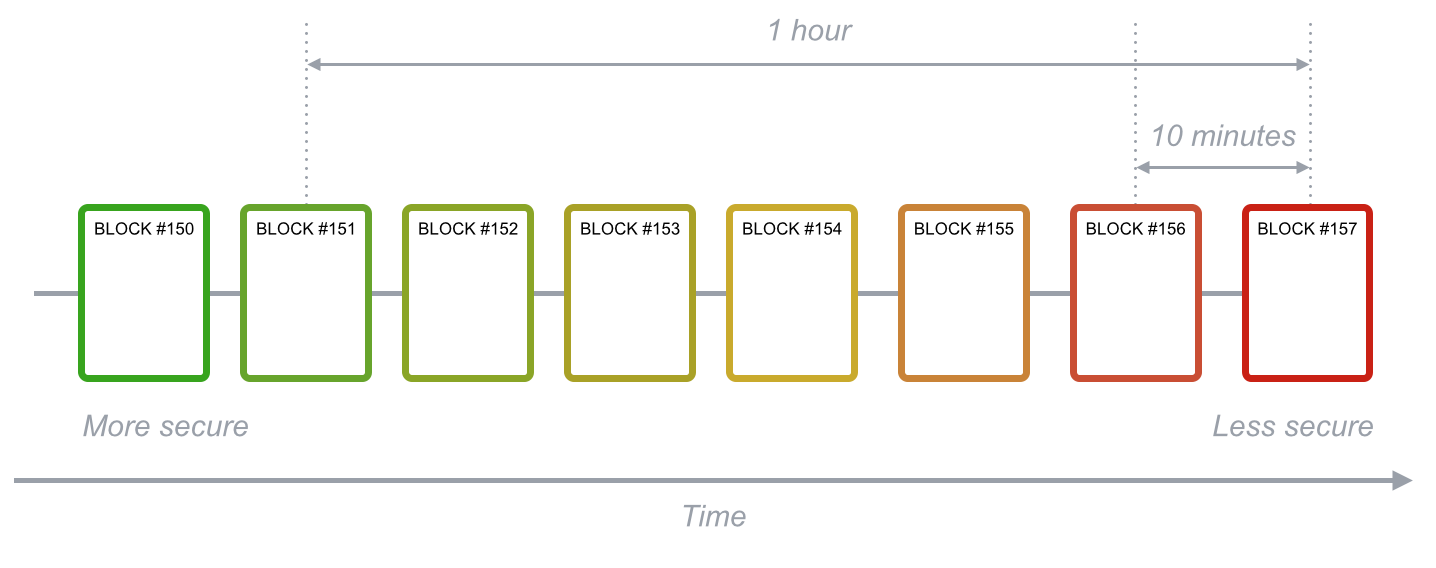
\includegraphics[scale=0.2]{bitcoin-security.png}
\end{frame}

\begin{frame}
    \frametitle{Two Generals' Problem}
    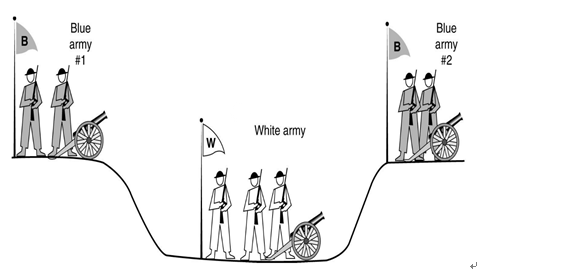
\includegraphics[scale=0.5]{two-generals-problem.png}
    \begin{itemize}
        \item \alert{Two generals} need to coordinate an attack.
            \begin{itemize}
                \item Must \alert{agree} on time to attack.
                \item They will win only if they attack \alert{simultaneously}.
                \item Communicate through \alert{messengers}.
                \item Messengers may be \alert{killed} on their way.
            \end{itemize}
    \end{itemize}
\end{frame}

\begin{frame}
    \frametitle{Two Generals' Problem}
    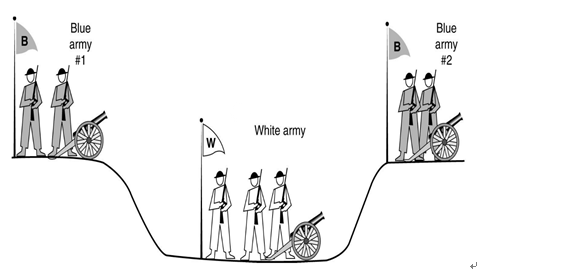
\includegraphics[scale=0.5]{two-generals-problem.png}
    \begin{itemize}
        \item Let's try to solve it for general g1 and g2.
        \item g1 sends \alert{time of attack} to g2.
            \begin{itemize}
                \item \alert{Problem}: how to ensure g2 received message?
                \item \alert{Solution}: let g2 ack receipt of message.
                \item \alert{Problem}: how to ensure g1 received ack?
                \item \alert{Solution}: let g1 ack the receipt of the ack.
                \item \ldots
            \end{itemize}
        \item This problem is \alert{impossible} to solve!
    \end{itemize}
\end{frame}

\begin{frame}
    \frametitle{Engineering approaches: TCP handshake}
    A progmatic approach to dealing with the Two Generals's Problem
    \begin{itemize}
        \item Accept the \alert{uncertainty} of the Communication channel.
        \item Not attempt to eliminate it, but mitigate it to an acceptable degree.
        \item Classic Example is TCP handshake protocol.
    \end{itemize}
    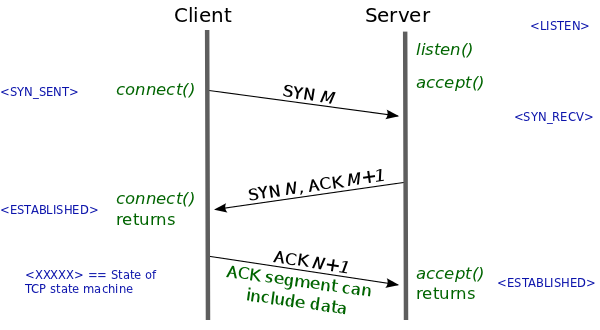
\includegraphics[scale=0.4]{tcp-handshake.png}
\end{frame}
